This section describes the performance results of HEPMiner and SCPMiner.
\subsection{HEPMiner Results}
In our experiments using HEPMiner, AFGMiner-locreg was always faster than AFGMiner-iso, and increasing the number of threads in p-AFGMiner consistently decreased run-time. As an example, when running with MMH and MinSup of 0.001, AFGMiner-iso took approximately 11 hours to complete the mining process, while AFGMiner-locreg took 40 minutes and p-AFGMiner with 8 threads took 15 minutes. The dramatic decrease in run-time when comparing AFGMiner-locreg to AFGMiner-iso is expected because location registration decreases the number of dataset sub-graphs that must be tested for isomorphism with candidate patterns. It causes the number of isomorphism tests to grow linearly with the number of candidate patterns, while in AFGMiner-iso it grows exponentially for general AFGs and polynomially for AFGs with bounded tree-width (such as EFGs). This observation led to our conjecture that the number of nodes visited when mining for each candidate pattern is the major factor determining the run-time of AFGMiner, as opposed to other factors such as the MaxAttrs. We tested this conjecture in Experiments {\bf A} and {\bf B} described in Section~\ref{sec:Methodology}, and the results are in Sub-section~\ref{subsec:Scalability}.

Memory consumption in HEPMiner is mostly determined by the size of $DS$. The support value has little influence, because the majority of candidate patterns are discarded, or, if considered heavyweight, deleted from memory when output to the user. The entire dataset, already in graph format, is kept in the RAM along with all mining-specific data structures. For very large datasets, another version of the tool could be developed that saves part of $DS$ to disk and retrieves parts of it when requested to do so by the mining algorithm.

We also compared patterns found by AFGMiner and FlowGSP. Figure~\ref{fig:NumPatterns} shows the number of output patterns for different MinSup values. As expected, AFGMiner found all patterns found by FlowGSP, but also found additional patterns composed of multiple sub-paths. For flat profiles, the trend is for AFGMiner to find many more patterns than FlowGSP as the MinSup is decreased, with the sequential patterns found by both being the parent patterns of the sub-graph patterns found exclusively by AFGMiner. 

\begin{figure}[h!]
\centering
    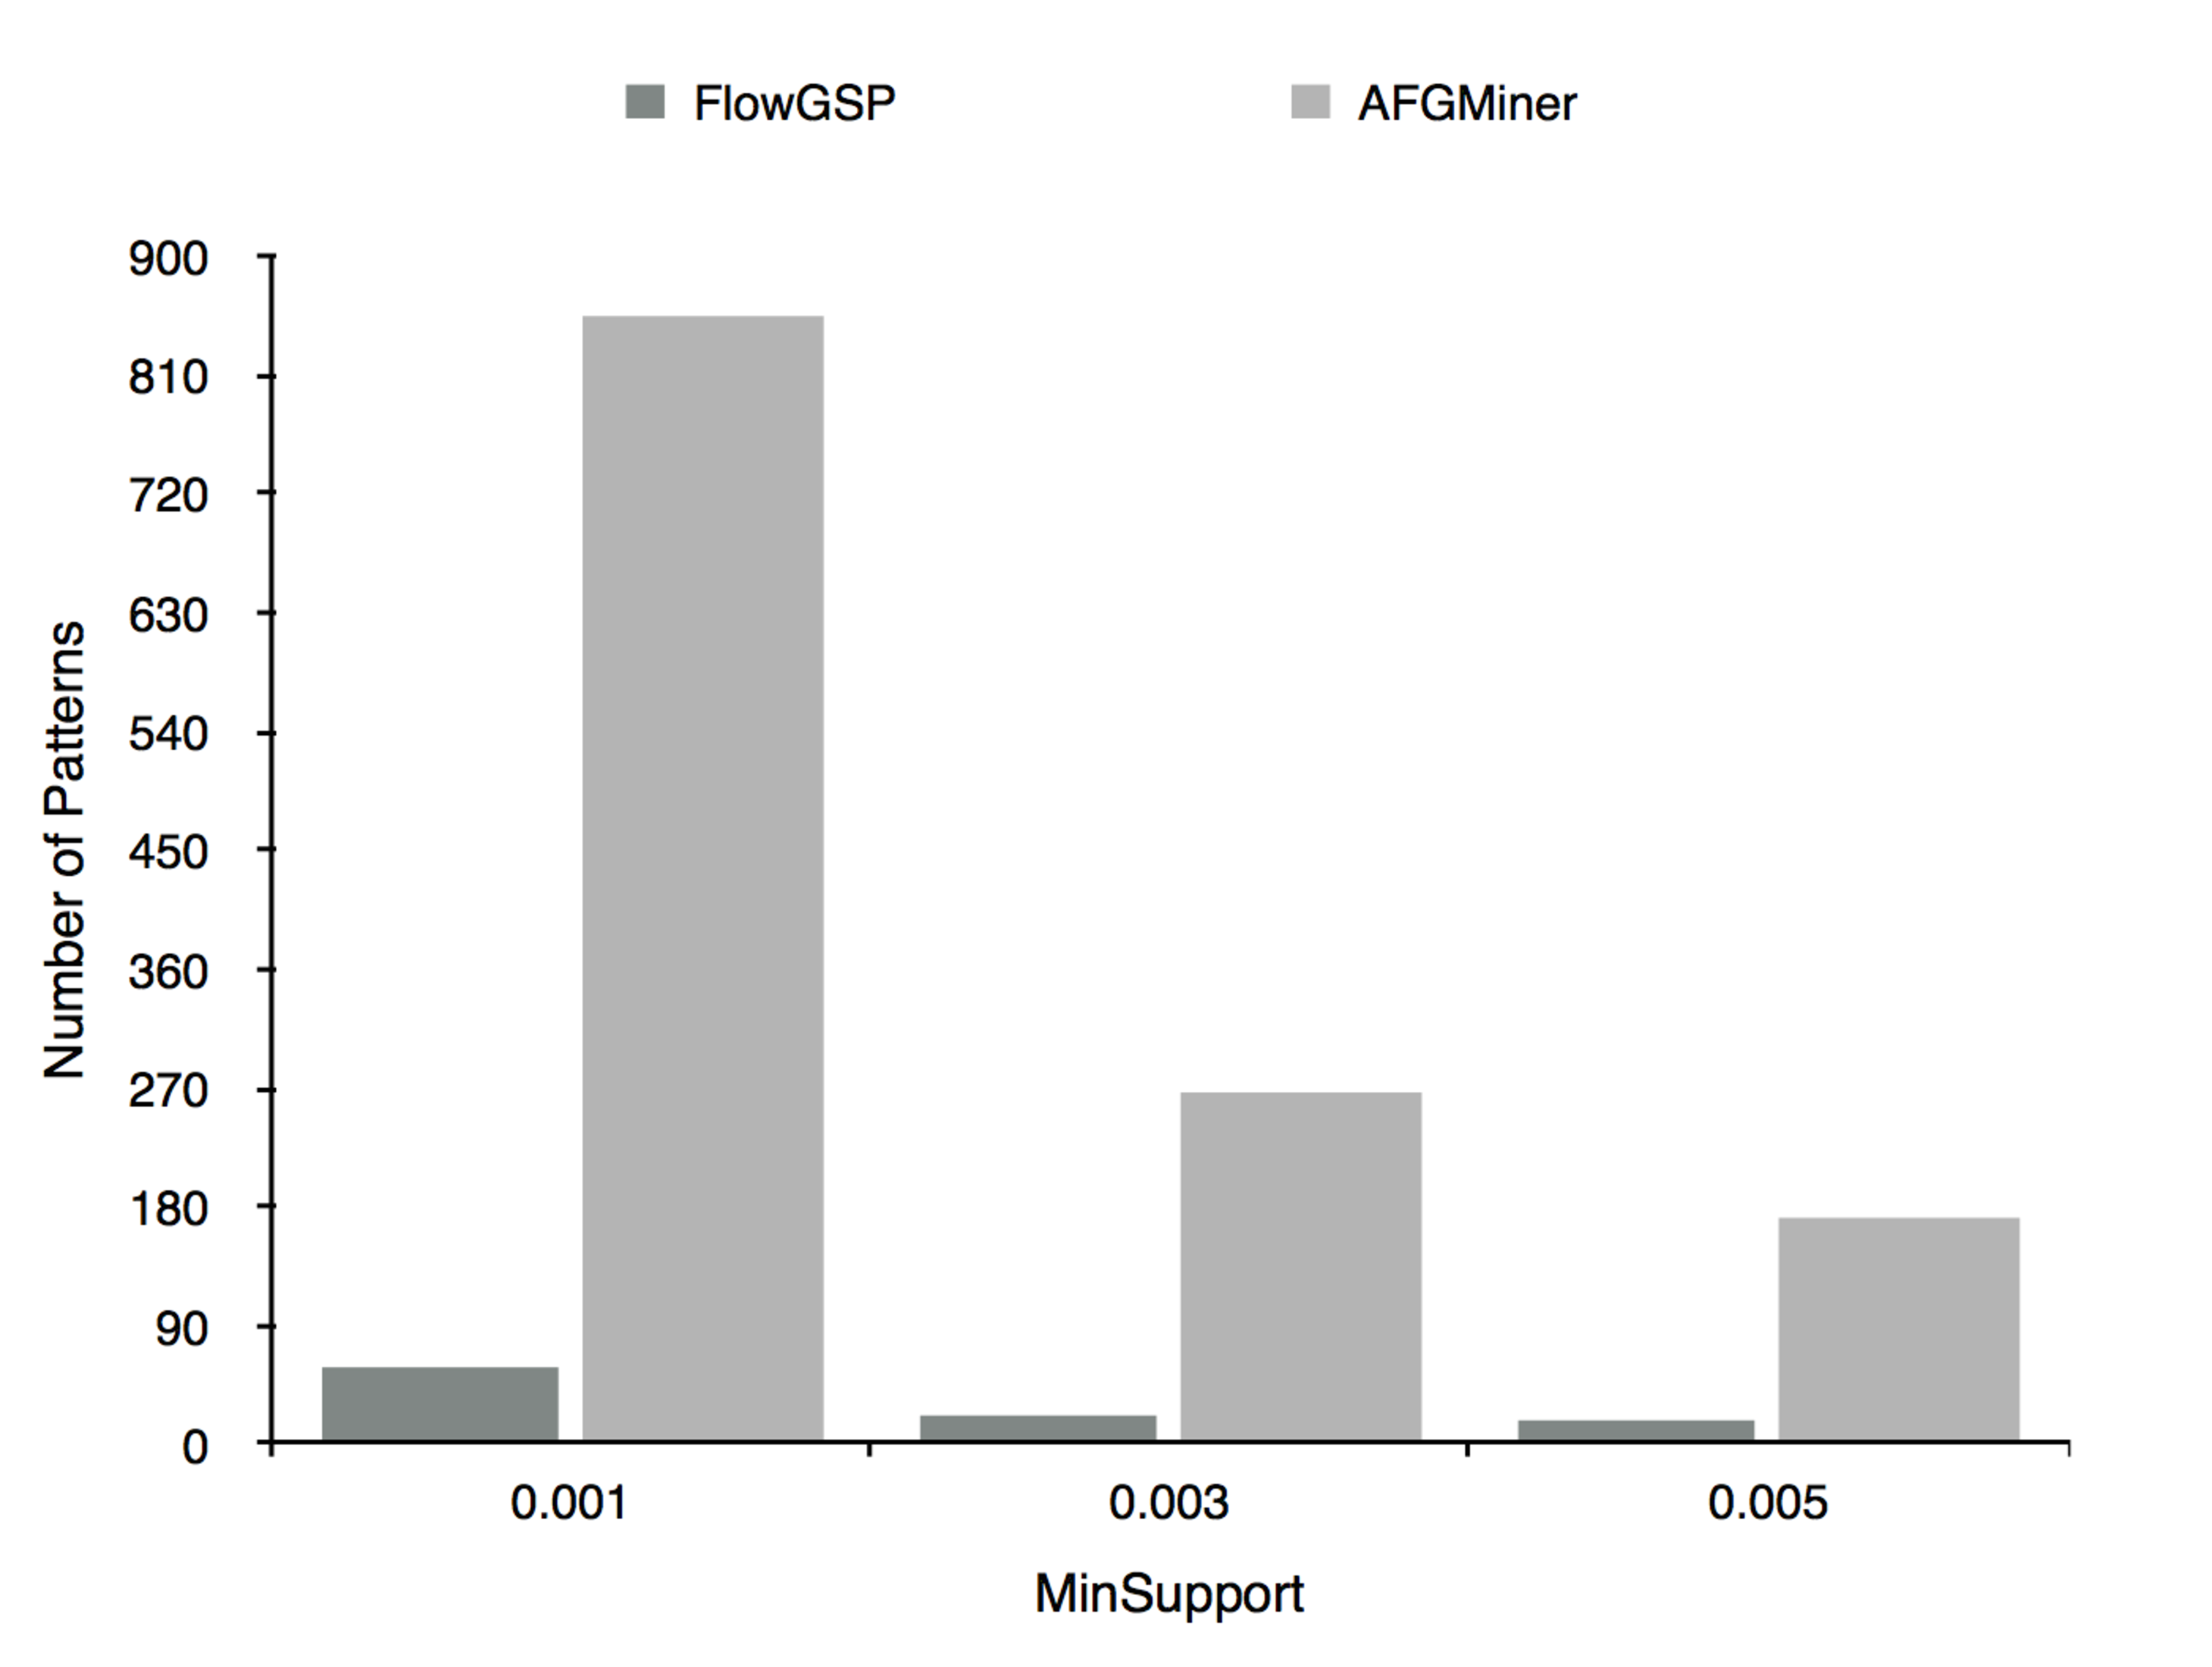
\includegraphics[scale=0.15]{figures/numPatternsComp.pdf}
    \caption{Patterns found by FlowGSP and AFGMiner}
    \label{fig:NumPatterns}
\end{figure}

\subsection{Scalability Analysis}
\label{subsec:Scalability}
From the results of Experiments {\bf A} (Figure~\ref{fig:Plot2}) and {\bf B} (Figure~\ref{fig:Plot1}) we conclude that the MaxAttrs value is not as relevant a factor in the run-time performance of AFGMiner as the number of EFG nodes visited during the mining process. Figure~\ref{fig:Plot2} shows that, in the DayTrader Benchmark, it is more likely that heavyweight patterns have around 7 attributes per node, because making MaxAttrs higher than 7 does not produce statistically significant differences in run-time. It is worth noting that the effects of MaxAttrs on the performance of AFGMiner is dependent on the program being analyzed. If the program's run-time behavior causes more hardware events to happen, then the influence of MaxAttrs is more visible.

Experiment {\bf B} changes the support value in order to increase the number of EFG nodes that the algorithm must visit. Figure~\ref{fig:Plot1} shows that the run-time of AFGMiner scales well enough with the number of EFG nodes visited. The performance of HEPMiner was deemed sufficient for it to be adopted as a handy tool by compiler developers in difficult analysis cases such as applications with flat profiles. However, better candidate pruning techniques could be developed to make AFGMiner faster. If more application-specific versions of the algorithm are developed in the future, those could take into account knowledge about which attributes are more likely to appear in the heavyweight patterns leading to more effective pruning of candidates.
\begin{figure}[h!]
\centering
    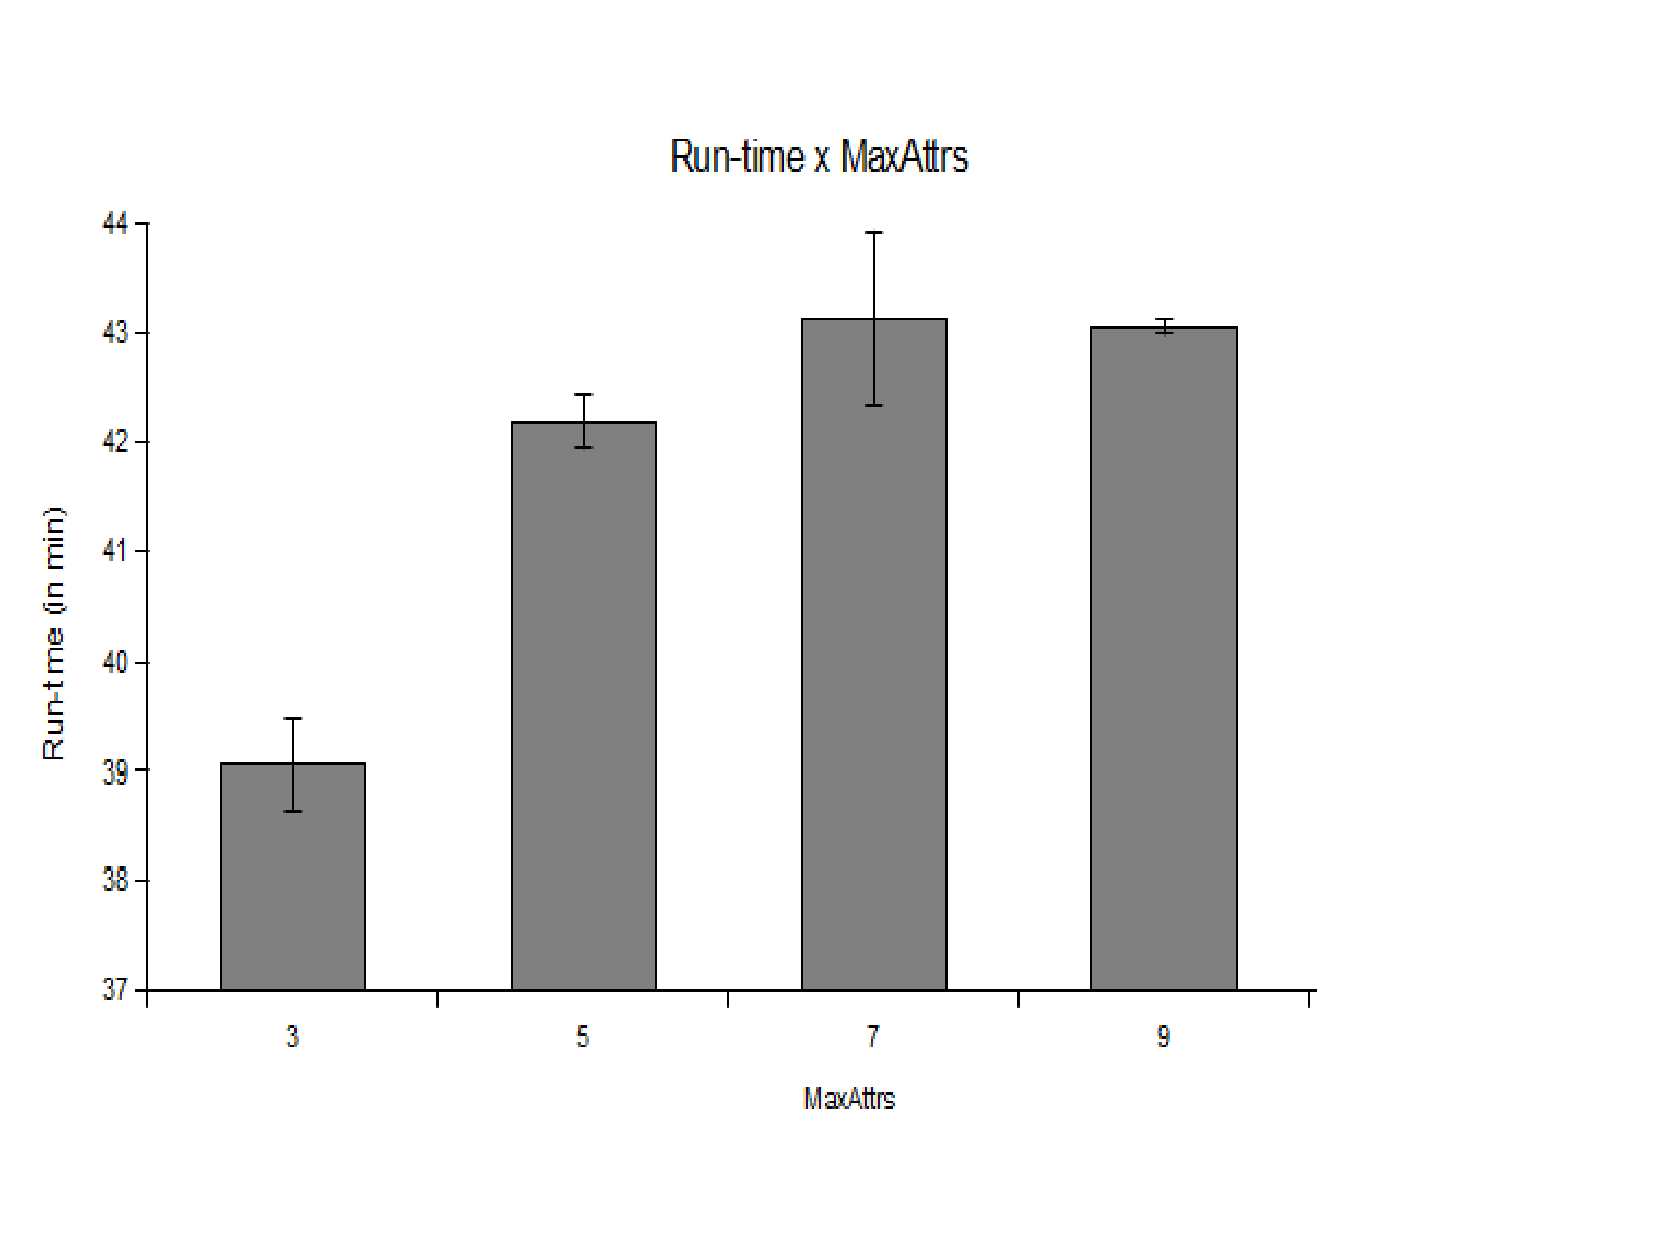
\includegraphics[scale=0.4]{figures/plot2.pdf}
    \caption{Experiment A.}
    \label{fig:Plot2}  
\end{figure}

\begin{figure}[h!]
\centering
    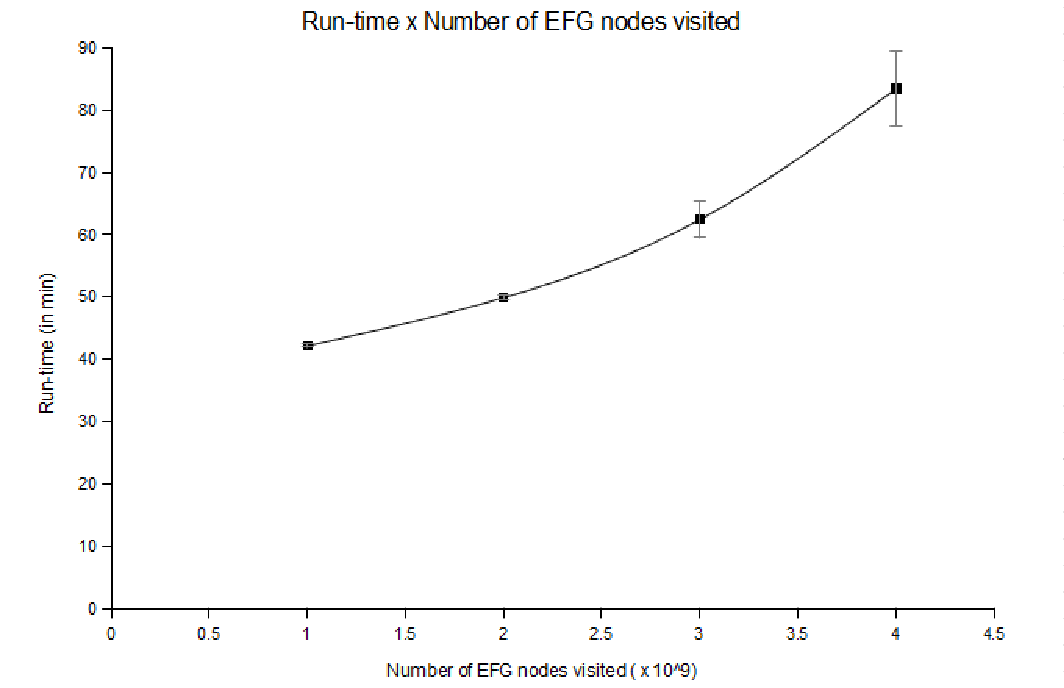
\includegraphics[scale=0.4]{figures/plot1.pdf}
    \caption{Experiment B.}
    \label{fig:Plot1}  
\end{figure}
